\chapter{Réalisation de la chaine de traitement.}

Je tiens ici à remercier le HIA Clermont Tonnerre de Brest et le CHRU de Brest pour m'avoir fourni les différentes IRMs de perfusion dont je vais vous montrer les résultats.

Quelque soit l'IRM considérée, la chaine de traitement restera la même. Il faudra choisir l'IRM d'un patient, stocker les images IRMs par coupe, choisir une coupe puis une région d'intérêt et enfin appliquer l'algorithme sur les éléments sélectionnés.

\begin{figure}[H]
\centering
    \includegraphics[scale=0.8,angle=0]{Images/Processing_toolchain.png}
    \caption{Chaine de traitement développée dans le cadre du projet.}
    \label{fig:toolchain}
\end{figure}

La sélection de la région d'intérêt se fait assez facilement avec Matlab comme le montre la figure suivante. L'idée est de prendre une zone et une coupe qui contiennent la zone présentant une pathologie.

\begin{figure}[H]
\centering
    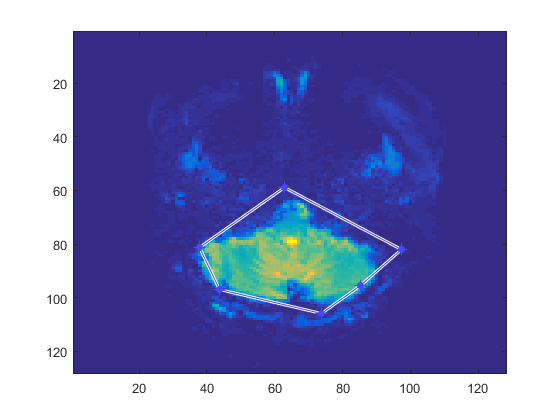
\includegraphics[scale=0.8,angle=0]{Images/ExampleROI.png}
    \caption{Choix d'une ROI avec Matlab.}
    \label{fig:ExampleROI}
\end{figure}


\chapter{IMRs T2 du crane CHRU Brest Cavale Blanche.}

Pendant ce PFE, j'ai pu récupérer une dizaine d'IRM de perfusion de cerveau présentant des lésions. La liste ci-dessous donne une liste des lésions considérées:

\begin{itemize}
\item Patient 2: Cancer visible sur les coupes 13 à 22.
\item Patient 6: * visible sur les coupes 5 à 9.
\item Patient 9: Lésion post-opératoire visible sur les coupes 15 à 19.
\end{itemize}

\begin{figure}[H]
\centering
\begin{subfigure}{.5\textwidth}
    \centering
    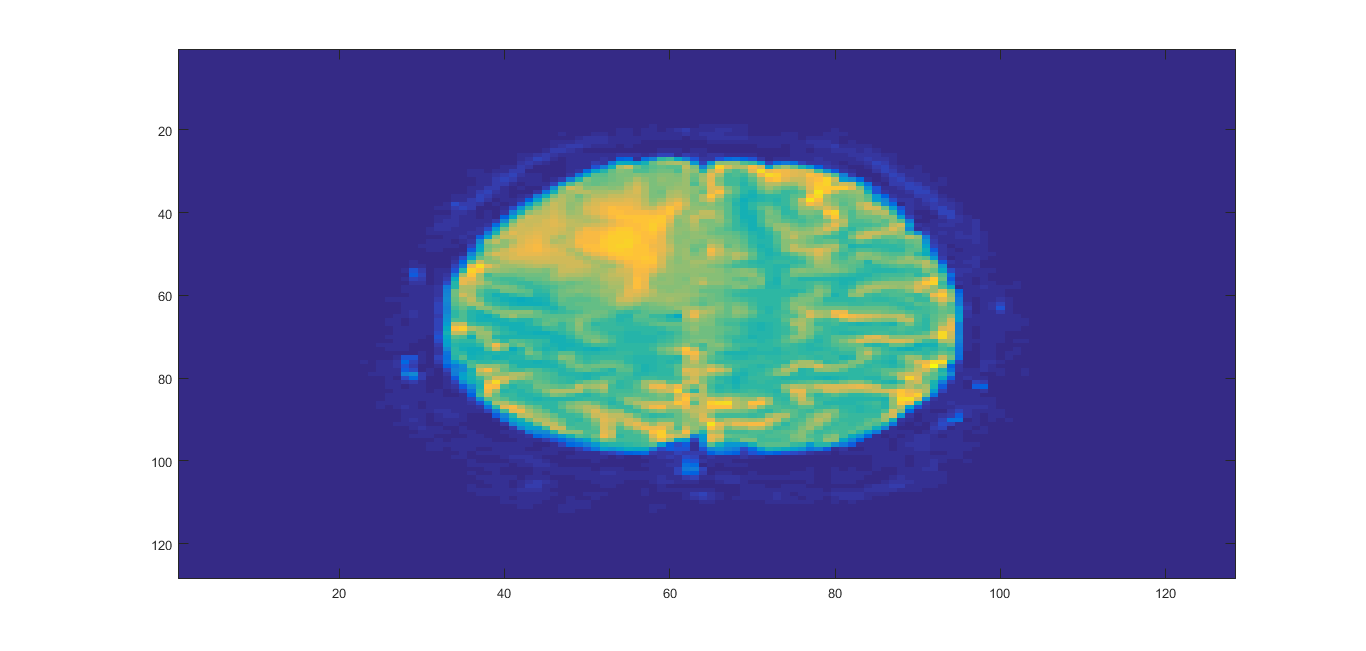
\includegraphics[scale=0.2,angle=0]{Images/TrueclassBrain.png}
    \caption{Image original.}
    \label{fig:TrueclassBrain} 
\end{subfigure}
\begin{subfigure}{.33\textwidth}
    \centering
    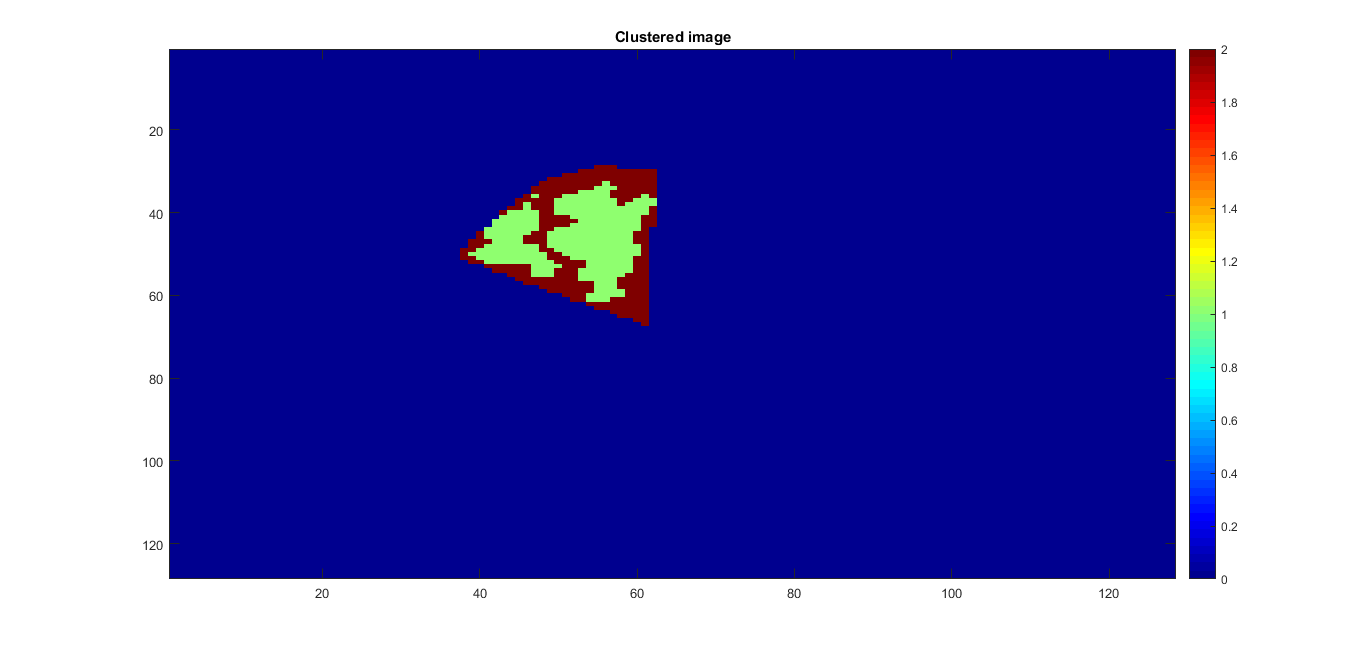
\includegraphics[scale=0.2,angle=0]{Images/2classBrain.png}
    \caption{2 classes.}
    \label{fig:2classBrain} 
\end{subfigure}
\begin{subfigure}{.33\textwidth}
    \centering
    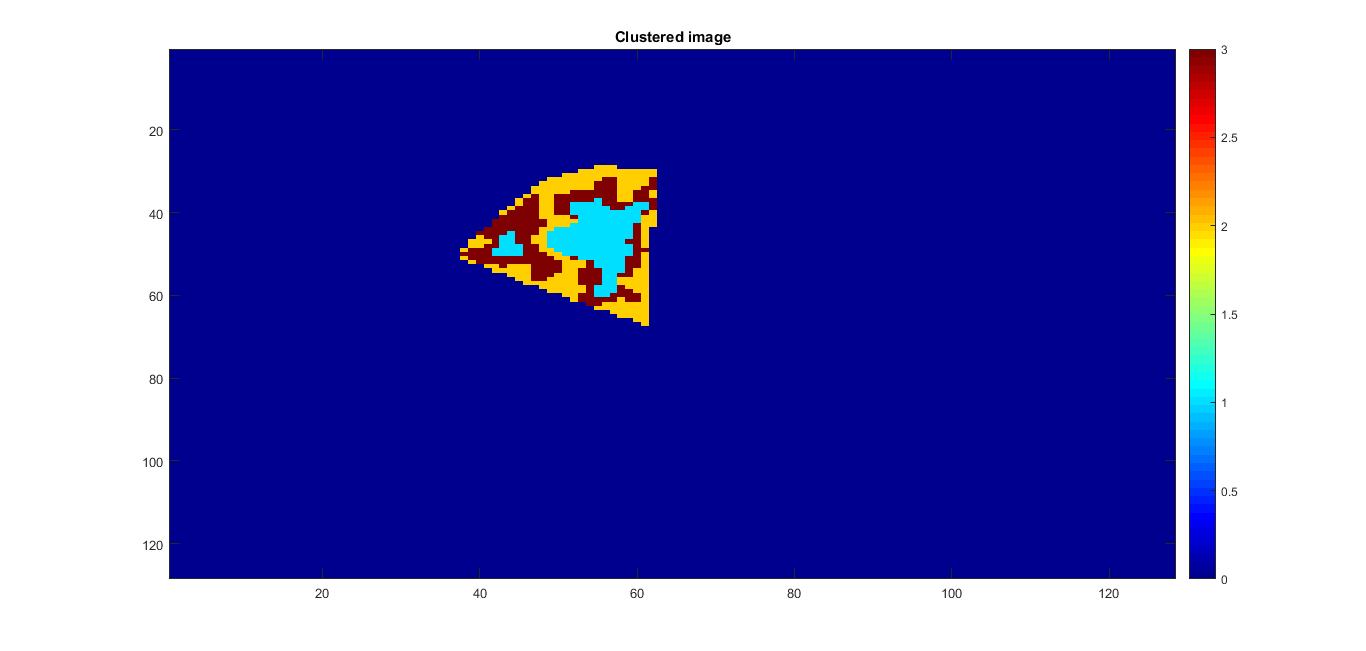
\includegraphics[scale=0.2,angle=0]{Images/3classBrain.png}
    \caption{3 classes.}
    \label{fig:3classBrain} 
\end{subfigure}
    \caption{Résultats de notre algorithme sur le patient 2 avec 2 et 3 classes.}
    \label{fig:2and3classBrain} 
\end{figure}









\chapter{IMRs T1 de la prostate de l'INSERM de Lille.}

\section{Types de courbe rencontrées dans le cadre du cancer de la prostate}

Une partie du travail qui est présenter ici peut être retrouver dans le lien suivant \cite{doi2007computer}.
Ce document présente les différentes courbes caractéristiques de la prostate. Les courbes d'intensité présentent toutes un hyper signal en IRM T1 mais les courbes issus de tissus cancéreux présentent un pic d'absorption beaucoup plus marqué avec un temps d'assimilation très caractéristique alors que les tissus sain présentent une courbe d'absorption beaucoup plus lissée. La figure suivant issu de \cite{doi2007computer} donne une illustration de ces courbes caractéristique.

\medskip

\begin{figure}[H]
\centering
    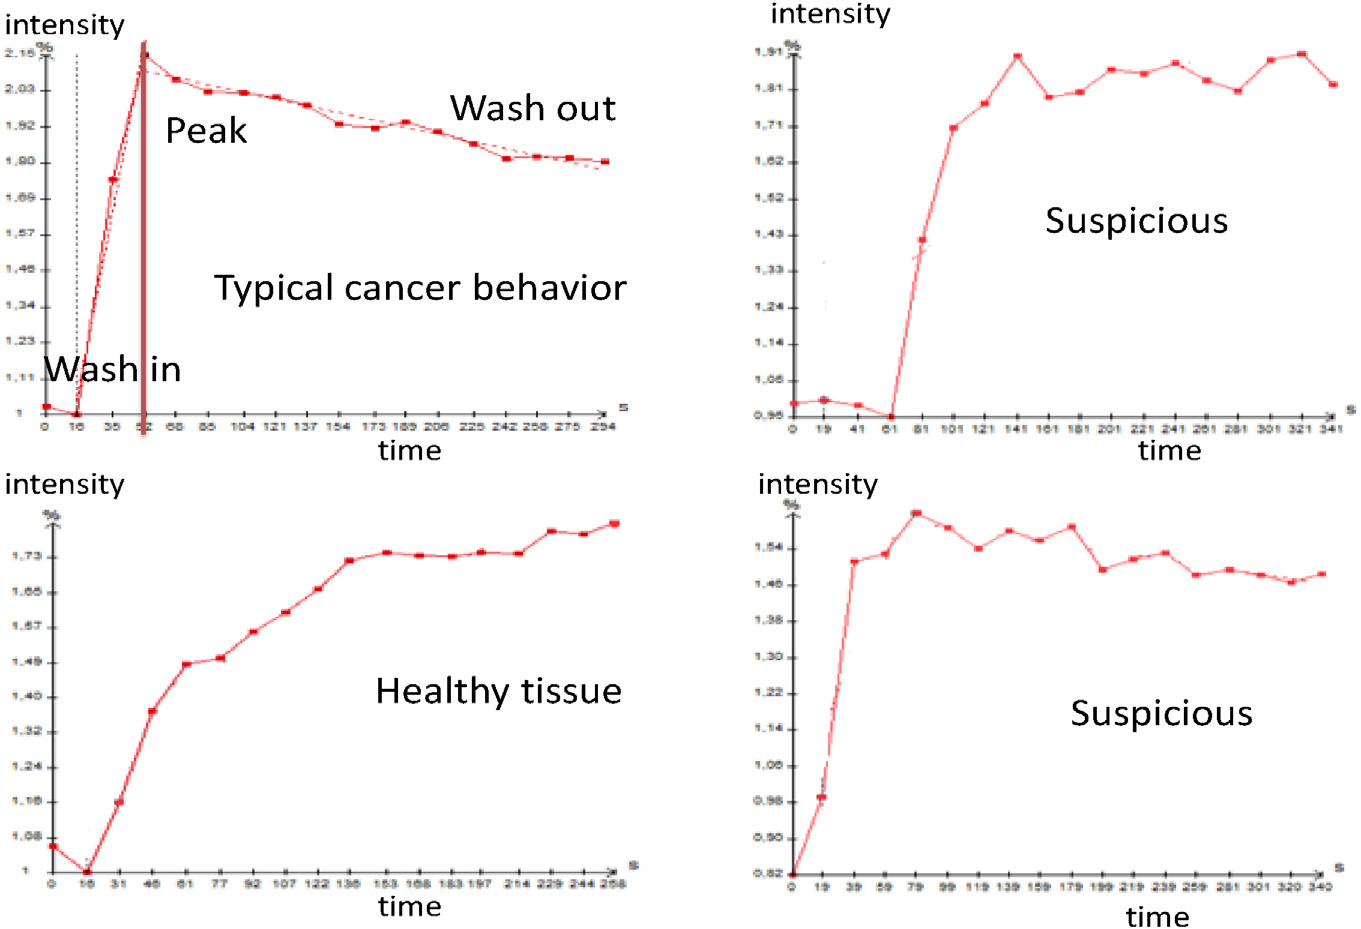
\includegraphics[scale=0.4,angle=0]{Images/CourbeProstate.png}
    \caption{Courbes caractéristiques des tissus sain et cancéreux de la prostate.}
    \label{fig:CourbeProstate}
\end{figure}

\medskip

Néanmoins, certaines courbes sont difficilement à classifier. L'intérêt de notre algorithme va donc être de pouvoir distinguer aisément les tissus sains et les tissus cancéreux et d'estimer avec une autre classe supplémentaire les cas d'incertitude.

\medskip

\textbf{\textcolor{blue}{ NOTA BENE}}: Dans le document précédent, il construise le graphe de similitude à partir de la similitude entre la courbe d'intensité du voxel considéré et de l'AIF. Chose qui n'est pas fait ici.


\section{Résultats de l'algorithme}

Pour appliquer nos algorithmes, il y a un petit pré-traitement à faire. Pour discriminer les différentes courbes, il faut surtout voir le phénomène de diffusion au sein du tissu et normaliser les courbes afin de faire ressortir le comportement du tissu.
\medskip

Tous les courbes sont donc remise à l'échelle en appliquant la formule suivante:

\begin{equation}
\centering
x(t) \gets \frac{x(t)-x_{min}}{x_{max}-x_{min}}
\end{equation} 

\medskip

Tous les signaux temporels sont donc placés dans une matrice comme expliqué dans la figure \ref{fig:toolchain}. 
Au final, en appliquant nos algorithmes à une IRM de perfusion de la prostate, nous arrivons au résultat suivant :

\begin{figure}[H]
\centering
    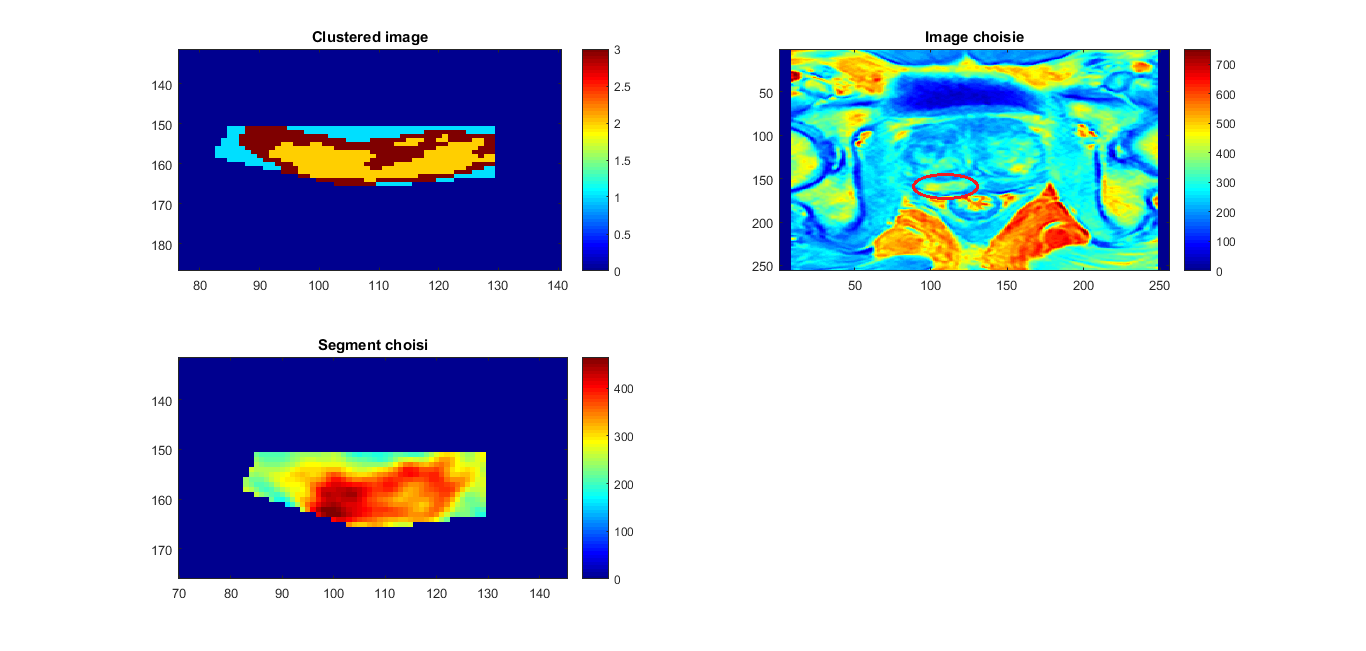
\includegraphics[scale=0.4,angle=0]{Images/3classProstate2.png}
    \caption{Coupes sélectionnées. En haut à gauche le résultat de l'algorithme de classification. En haut à droit, image de la coupe sélectionnée avec la ROI représentée par l'ellipse rouge. En bas à gauche, ROI en fausses couleurs.}
    \label{fig:3classProstate2}
\end{figure} 

La figure suivante montre comment les courbes sont réparties selon les différents clusters.

\begin{figure}[H]
\centering
    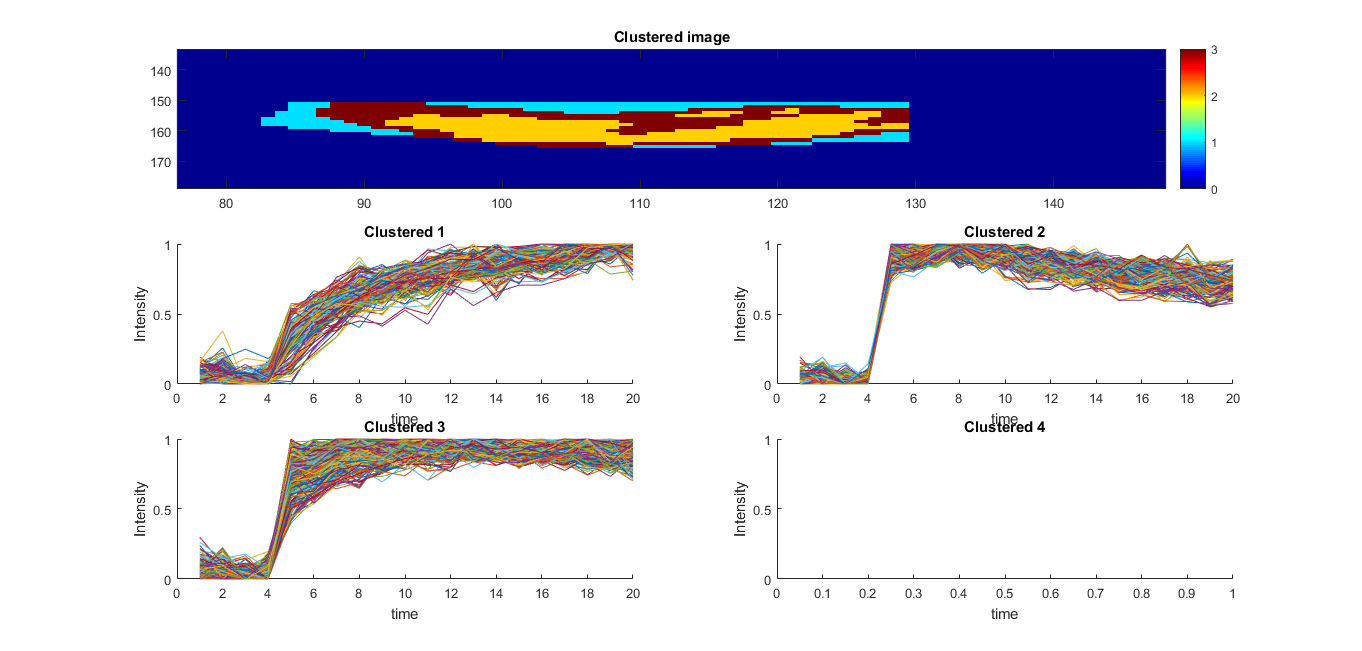
\includegraphics[scale=0.4,angle=0]{Images/3classProstate.png}
    \caption{Résultat de l'algorithme sur l'IRM avec les courbes associées aux clusters.}
    \label{fig:3classProstate}
\end{figure}

Nous avons ici lancé une simulation avec 3 classes. Nous pouvons interpréter ces résultats de la façon suivante:

\begin{itemize}
\item Le cluster 1 rassemble les courbes qui sont saines en accord avec les informations issus de la figure \ref{fig:CourbeProstate}
\item Le cluster 2 lui rassemble les courbes des tissus tumoraux qui présentent un temps d'absorption très court et un pic très marqué.
\item Le cluster 3 lui représentent des courbes qui sont à mis chemin entre les deux autres courbes caractéristiques. Ici, l'algorithme comme l'humain va avoir du mal à trancher sur l'appartenance de ces tissus au cluster sain ou tumoral.
\end{itemize}

Ici, on arrive à un résultat en partie semblable au médecin qui a à analyser ces images. On arrive à identifier de façon claire la zone tumoral et la zone litigieuse qui est assez souvent traitement de la même manière.

Néanmoins, il y a quelques remarques à faire:

\begin{itemize}
\item Il faut parfois choisir une bonne représentation des données de départ afin que l'algorithme converge vers une solution satisfaisante.
\item Il est nécessaire de choisir une ROI qui est composé d'une zone homogène et de préférence de taille pas trop importante. En effet, l'algorithme ne converge pas si il y a trop de point sélectionné.
\item Il y a un grand enjeu sur la détermination automatique du nombre de classe mais ceci sera plus longtemps abordé dans la partie 4.
\end{itemize}






